\documentclass[aspectratio=169, 10pt]{beamer}

% Theme and Color Scheme
\usetheme{Madrid}
\usecolortheme{whale}

% Standard Packages
\usepackage[utf8]{inputenc}
\usepackage{amsmath, amssymb, amsfonts}
\usepackage{graphicx}
\usepackage{booktabs}
\usepackage{multirow}
\usepackage{array}
\usepackage{tikz}
\usepackage{hyperref}
\usepackage{colortbl}
\usepackage{tcolorbox}

% Beamer Customizations
\setbeamertemplate{navigation symbols}{}
\setbeamertemplate{caption}[numbered]
\setbeamerfont{title}{size=\large, series=\bfseries}
\setbeamerfont{frametitle}{size=\normalsize, series=\bfseries}
\setbeamercolor{block title}{bg=blue!80!black, fg=white}
\setbeamercolor{block body}{bg=blue!5!white}

% Custom Colors
\definecolor{navyblue}{RGB}{20, 45, 95}
\definecolor{darkgreen}{RGB}{25, 115, 60}
\definecolor{alertred}{RGB}{185, 30, 30}
\definecolor{tableheader}{RGB}{220, 230, 242}

% Title and Metadata
\title[IDS Placement in RPL: Federated Learning Approach]{Exploring and Enhancing Placement of Intrusion Detection Systems in RPL: A Federated Learning-Based Approach}
\subtitle{Course Project: Computer Networks and Security (CNS) -- Team 19}
\author[Team 19]{Mohammadilyas Patel (CS23B1078) \\ Shaik Sifat Ahmed (CS23B1035) \\ Abhinay (CS23I1009)}
\institute[IIITDM Kancheepuram]{
  Department of Computer Science and Engineering \\
  Indian Institute of Information Technology, Design and Manufacturing, Kancheepuram \\
  Repository: \url{https://github.com/mdilyas-27/cns_project_team19}
}
\date{\today}

\begin{document}

% ==============================================================================
% SLIDE 1: TITLE SLIDE
% ==============================================================================
\begin{frame}
  \titlepage
  \begin{center}
    \footnotesize
    \textit{Based on Research by Selim Y{\i}lmaz, Sevil Sen, and Emre Aydogan (IEEE Internet of Things Journal, 2025)}
  \end{center}
\end{frame}

% ==============================================================================
% SLIDE 2: OVERVIEW / AGENDA
% ==============================================================================
\begin{frame}{Overview / Presentation Agenda}
  \tableofcontents
\end{frame}

% ==============================================================================
% SLIDE 3: BACKGROUND
% ==============================================================================
\section{Background}
\begin{frame}{Background: RPL in Low-Power \& Lossy Networks (LLNs)}
  \begin{columns}[T]
    \begin{column}{0.55\textwidth}
      \textbf{Routing Protocol for LLNs (RPL -- RFC 6550):}
      \begin{itemize}
        \item Tailored for constrained IoT devices (limited CPU, 8--10~KB RAM, battery-driven).
        \item Builds a \textbf{DODAG} (Destination-Oriented Directed Acyclic Graph) rooted at a border router / sink node.
        \item Utilizes Objective Functions (\textbf{OF0}, \textbf{MRHOF}) to compute node \textbf{Rank} based on link metrics (e.g., Expected Transmission Count, ETX).
      \end{itemize}
      \vspace{0.2cm}
      \textbf{RPL Control Messages:}
      \begin{itemize}
        \item \textbf{DIO} (DODAG Information Object): Upward routing advertisement.
        \item \textbf{DIS} (DODAG Information Solicitation): Probe for DODAG.
        \item \textbf{DAO} / \textbf{DAO-ACK}: Downward route establishment.
      \end{itemize}
    \end{column}
    \begin{column}{0.43\textwidth}
      \begin{figure}
        \centering
        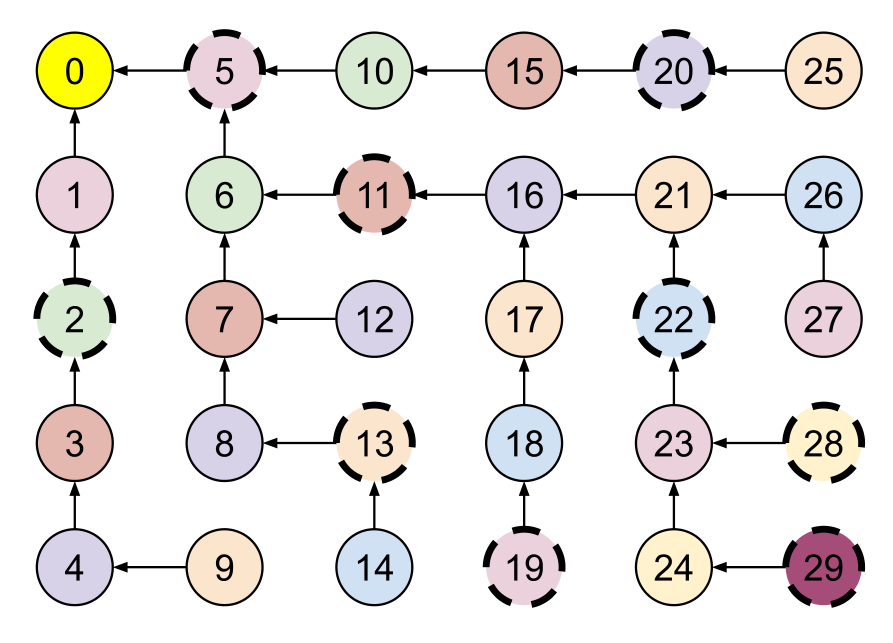
\includegraphics[width=\textwidth]{images/fig1_network_topology.png}
        \caption{Grid DODAG topology (30 nodes, 10 levels) \cite{yilmaz2025exploring}.}
      \end{figure}
    \end{column}
  \end{columns}
\end{frame}

% ==============================================================================
% SLIDE 4: RESEARCH GAP
% ==============================================================================
\section{Research Gap}
\begin{frame}{Research Gap in Existing IoT Intrusion Detection}
  \begin{columns}[T]
    \begin{column}{0.5\textwidth}
      \begin{block}{Limitations of State-of-the-Art Literature}
        \begin{itemize}
          \item \textbf{Heavy Algorithm Bias:} Literature proposes complex classifiers (SVM, RF, Deep Learning) but assumes an \textit{idealized central observer}.
          \item \textbf{Ignored Physical/Logical Placement:} The spatial distance between attacker and IDS node across multi-hop DAG levels has been largely unstudied.
          \item \textbf{Unrealistic Communication Assumptions:} Centralized models require streaming high-frequency raw features, congesting lossy 802.15.4 channels.
        \end{itemize}
      \end{block}
    \end{column}
    \begin{column}{0.48\textwidth}
      \begin{block}{Critical Open Questions Addressed}
        \begin{itemize}
          \item Does an IDS placed at the root detect attacks occurring 5--8 hops away at deep DAG levels?
          \item How does collaborator density impact detection vs. battery exhaustion?
          \item How can nodes cooperatively detect intrusions without centralizing private network traffic data?
        \end{itemize}
      \end{block}
      \begin{alertblock}{Identified Research Void}
        Lack of a systematic multi-criteria benchmark (Accuracy, Overhead, Latency, Privacy, Resilience) evaluating \textbf{IDS Placement} in RPL topologies.
      \end{alertblock}
    \end{column}
  \end{columns}
\end{frame}

% ==============================================================================
% SLIDE 5: MOTIVATION
% ==============================================================================
\section{Motivation}
\begin{frame}{Motivation: Why IDS Placement \& Decentralization Matter}
  \begin{columns}[T]
    \begin{column}{0.5\textwidth}
      \textbf{Vulnerability to Insider Threats:}
      \begin{itemize}
        \item Constrained nodes deployed in unattended areas can be physically captured or compromised.
        \item Legitimate cryptographic keys cannot prevent an insider from dropping packets or broadcasting malicious routing ranks.
      \end{itemize}
      \vspace{0.2cm}
      \textbf{Severe Resource Constraints:}
      \begin{itemize}
        \item Sensor motes (e.g., Zolertia Z1) have severe energy budgets.
        \item Continuous multi-hop telemetry drains node batteries and induces packet collisions.
      \end{itemize}
    \end{column}
    \begin{column}{0.48\textwidth}
      \begin{figure}
        \centering
        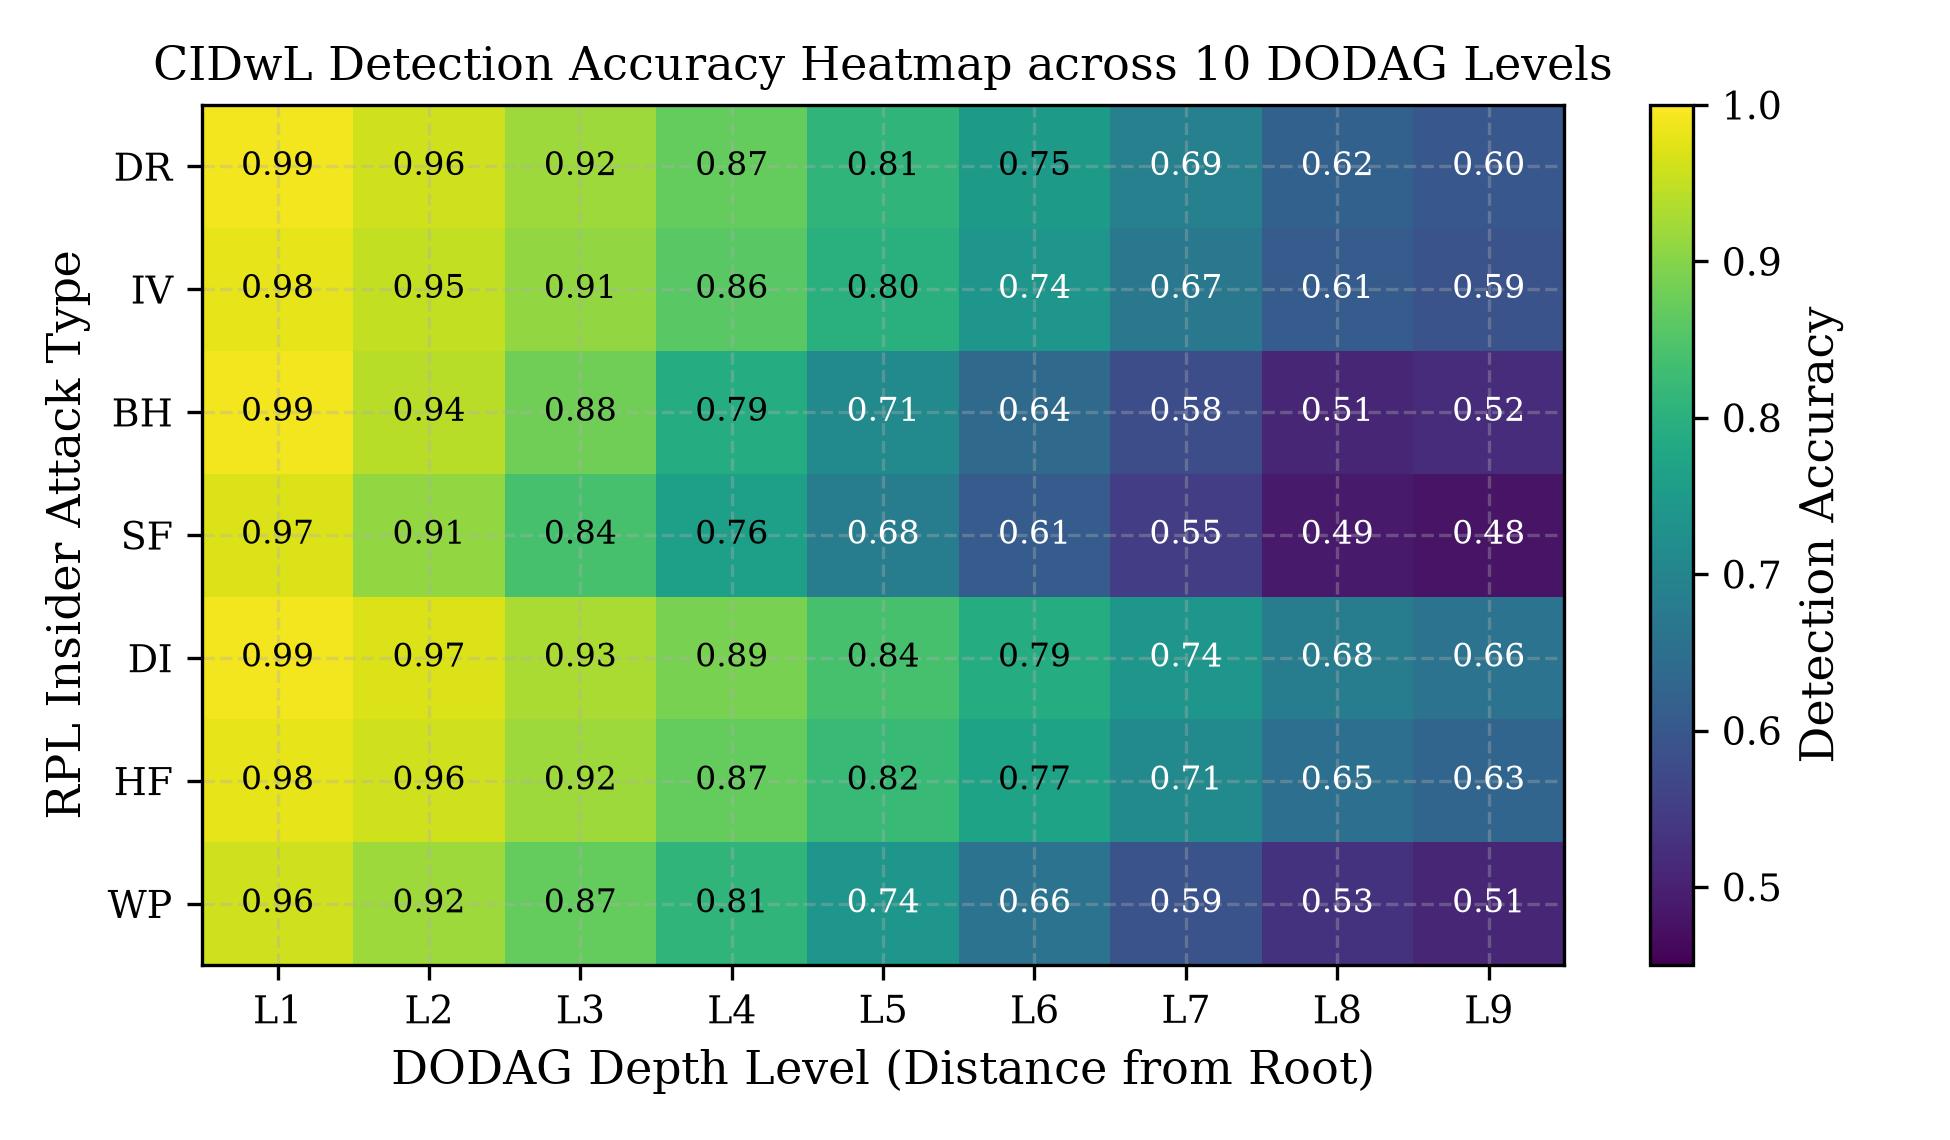
\includegraphics[width=\textwidth]{images/fig3_detection_accuracy_heatmap.png}
        \caption{Detection accuracy heatmap showing spatial degradation with distance \cite{yilmaz2025exploring}.}
      \end{figure}
      \vspace{-0.3cm}
      \begin{exampleblock}{Core Motivation}
        Design an intrusion detection framework that guarantees \textbf{high multi-hop accuracy} while eliminating runtime communication overhead and preserving node privacy.
      \end{exampleblock}
    \end{column}
  \end{columns}
\end{frame}

% ==============================================================================
% SLIDE 6: OBJECTIVES
% ==============================================================================
\section{Objectives}
\begin{frame}{Project Objectives \& Research Questions}
  \begin{block}{Primary Research Questions (RQs)}
    \begin{description}
      \item[\textbf{RQ1:}] \textit{Is one central IDS enough for effectively detecting all types of attacks performed at different topological locations?}
      \item[\textbf{RQ2:}] \textit{What is the minimum number and distribution of IDS nodes required for effective network-wide detection?}
      \item[\textbf{RQ3:}] \textit{How can IDSs make collective decisions efficiently from a communication cost perspective?}
    \end{description}
  \end{block}
  \vspace{0.2cm}
  \begin{columns}[T]
    \begin{column}{0.48\textwidth}
      \textbf{Evaluation Objectives:}
      \begin{itemize}
        \item Rigorously benchmark three baseline architectures across 31,626 simulation scenarios:
          \begin{enumerate}
            \item Centralized ID with Local Info (\textbf{CIDwL})
            \item Centralized ID with Global Info (\textbf{CIDwG})
            \item Distributed Collaborative ID (\textbf{DCID})
          \end{enumerate}
      \end{itemize}
    \end{column}
    \begin{column}{0.48\textwidth}
      \textbf{Proposed Solution \& Novelty:}
      \begin{itemize}
        \item Implement \textbf{FedID}: A Federated Learning-based IDS leveraging XGBoost and FedAvg \cite{yilmaz2025exploring}.
        \item Propose \textbf{Next-Iteration Novelty}: Dynamic Adaptive IDS Placement with Byzantine Resilience and Local Differential Privacy.
      \end{itemize}
    \end{column}
  \end{columns}
\end{frame}

% ==============================================================================
% SLIDE 7: EXPERIMENTAL SETUP
% ==============================================================================
\section{Experimental Setup}
\begin{frame}{Experimental Setup \& Simulation Environment}
  \begin{columns}[T]
    \begin{column}{0.5\textwidth}
      \begin{table}[h]
        \centering
        \scriptsize
        \caption{Simulation Configuration Parameters \cite{yilmaz2025exploring}}
        \begin{tabular}{ll}
          \toprule
          \textbf{Parameter} & \textbf{Value} \\
          \midrule
          Simulator & Cooja (Contiki OS 2.7) \\
          Mote Platform & Zolertia Z1 (MSP430 MCU, 8KB RAM) \\
          Radio Model & UDGM: Distance Loss \\
          TX / Carrier Range & 25 m / 50 m \\
          Deployment Area & $100\text{ m} \times 80\text{ m}$ Grid \\
          Node Count & 30 nodes (1 Root / Sink, 29 Sensors) \\
          DODAG Levels & 10 Levels (Hop distance 1 to 9) \\
          Objective Function & MRHOF (Metric: ETX) \\
          Traffic Pattern & Periodic UDP (1 pkt / 15 s) \\
          Simulation Duration & 5 hours per scenario \\
          Total Scenarios & 31,626 distinct evaluations \\
          \bottomrule
        \end{tabular}
      \end{table}
    \end{column}
    \begin{column}{0.48\textwidth}
      \textbf{Seven Targeted RPL Attacks:}
      \begin{enumerate}\scriptsize
        \item \textbf{Decreased Rank (DR):} Illegitimate low rank advertising to hijack downward routes.
        \item \textbf{Increased Version (IV):} Unauthorized version churn triggering global rebuilding loops.
        \item \textbf{Blackhole (BH):} Silent dropping of all intercepted forwarding packets.
        \item \textbf{Selective Forwarding (SF):} Probabilistic dropping of specific data packets.
        \item \textbf{DIS Flooding (DI):} Continuous solicitation resetting neighbor trickle timers.
        \item \textbf{DIO / Hello Flooding (HF):} High-frequency routing broadcast exhausting energy.
        \item \textbf{Wormhole / P2P Bypass (WP):} Out-of-band tunnel bypassing legitimate hops.
      \end{enumerate}
    \end{column}
  \end{columns}
\end{frame}

% ==============================================================================
% SLIDE 8: DATASET
% ==============================================================================
\section{Dataset}
\begin{frame}{Dataset \& Feature Engineering}
  \begin{columns}[T]
    \begin{column}{0.52\textwidth}
      \textbf{Network-Layer Traffic Feature Extraction:}
      \begin{itemize}
        \item \textbf{Time Windowing:} Continuous traffic segmented into \textbf{60-second non-overlapping windows}.
        \item \textbf{35 Features Extracted \cite{yilmaz2021transfer}:}
          \begin{itemize}\footnotesize
            \item Packet frequency: DIO, DIS, DAO transmitted/received.
            \item Data traffic rate: forwarded vs. dropped ratios.
            \item Protocol fields: Rank stability, Version numbers.
            \item Timing metrics: Inter-arrival time mean and variance.
          \end{itemize}
        \item \textbf{Non-IID Characteristics:}
          Traffic distribution differs drastically by DODAG depth (leaf nodes generate minimal traffic; root transit nodes experience high traffic density).
      \end{itemize}
    \end{column}
    \begin{column}{0.46\textwidth}
      \textbf{Benchmark Validation Dataset:}
      \begin{block}{CICIoT2023 Real-Time Dataset \cite{neto2023ciciot2023}}
        \begin{itemize}\footnotesize
          \item Real-world large-scale IoT traffic benchmark.
          \item \textbf{33 attack types} grouped into 7 main categories: DDoS, DoS, Reconnaissance, Web, Brute-Force, Spoofing, Mirai.
          \item Used to evaluate binary and 34-class multiclass generalization.
        \end{itemize}
      \end{block}
      \begin{figure}
        \centering
        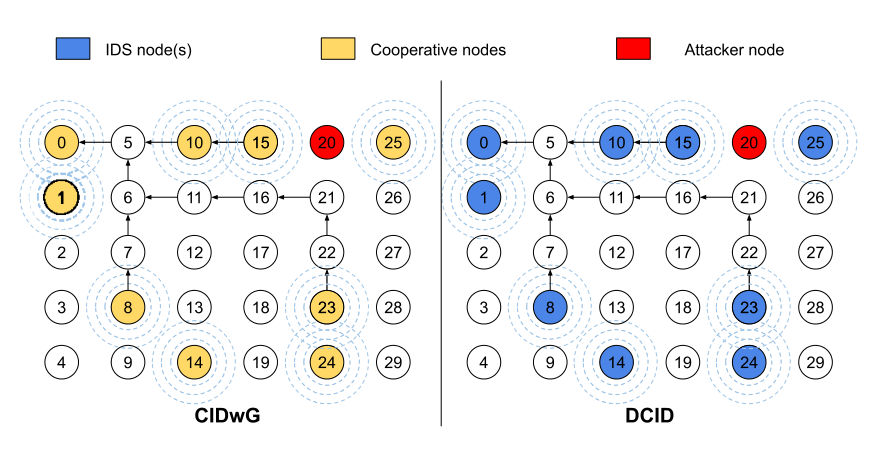
\includegraphics[width=\textwidth]{images/fig2_scenario_collaborators.png}
        \caption{Collaborator deployment across DAG levels \cite{yilmaz2025exploring}.}
      \end{figure}
    \end{column}
  \end{columns}
\end{frame}

% ==============================================================================
% SLIDE 9: RESULTS PART 1
% ==============================================================================
\section{Results: Architectural Comparison}
\begin{frame}{Results (Part 1): Architectural Placement Analysis (RQ1 \& RQ2)}
  \begin{columns}[T]
    \begin{column}{0.52\textwidth}
      \textbf{Answer to RQ1 (Single Central IDS):}
      \begin{itemize}\footnotesize
        \item \textbf{CIDwL is Insufficient:} Detection collapses when attacks occur far from the root (e.g., Blackhole drops from 98.8\% at Level 1 to 51.5\% at Level 8).
        \item Selective Forwarding (SF) max accuracy is only 58.0\%!
      \end{itemize}
      \vspace{0.1cm}
      \textbf{Answer to RQ2 (Minimum Collaborators):}
      \begin{itemize}\footnotesize
        \item \textbf{CIDwG Placement:} Enrolling at least 1 collaborator per DODAG level restores detection (BH jumps from 78.3\% with 2 nodes to 99.4\% with 9 nodes).
        \item 9 collaborators achieve 99.9\% on HF and 100\% on IV.
      \end{itemize}
    \end{column}
    \begin{column}{0.46\textwidth}
      \begin{figure}
        \centering
        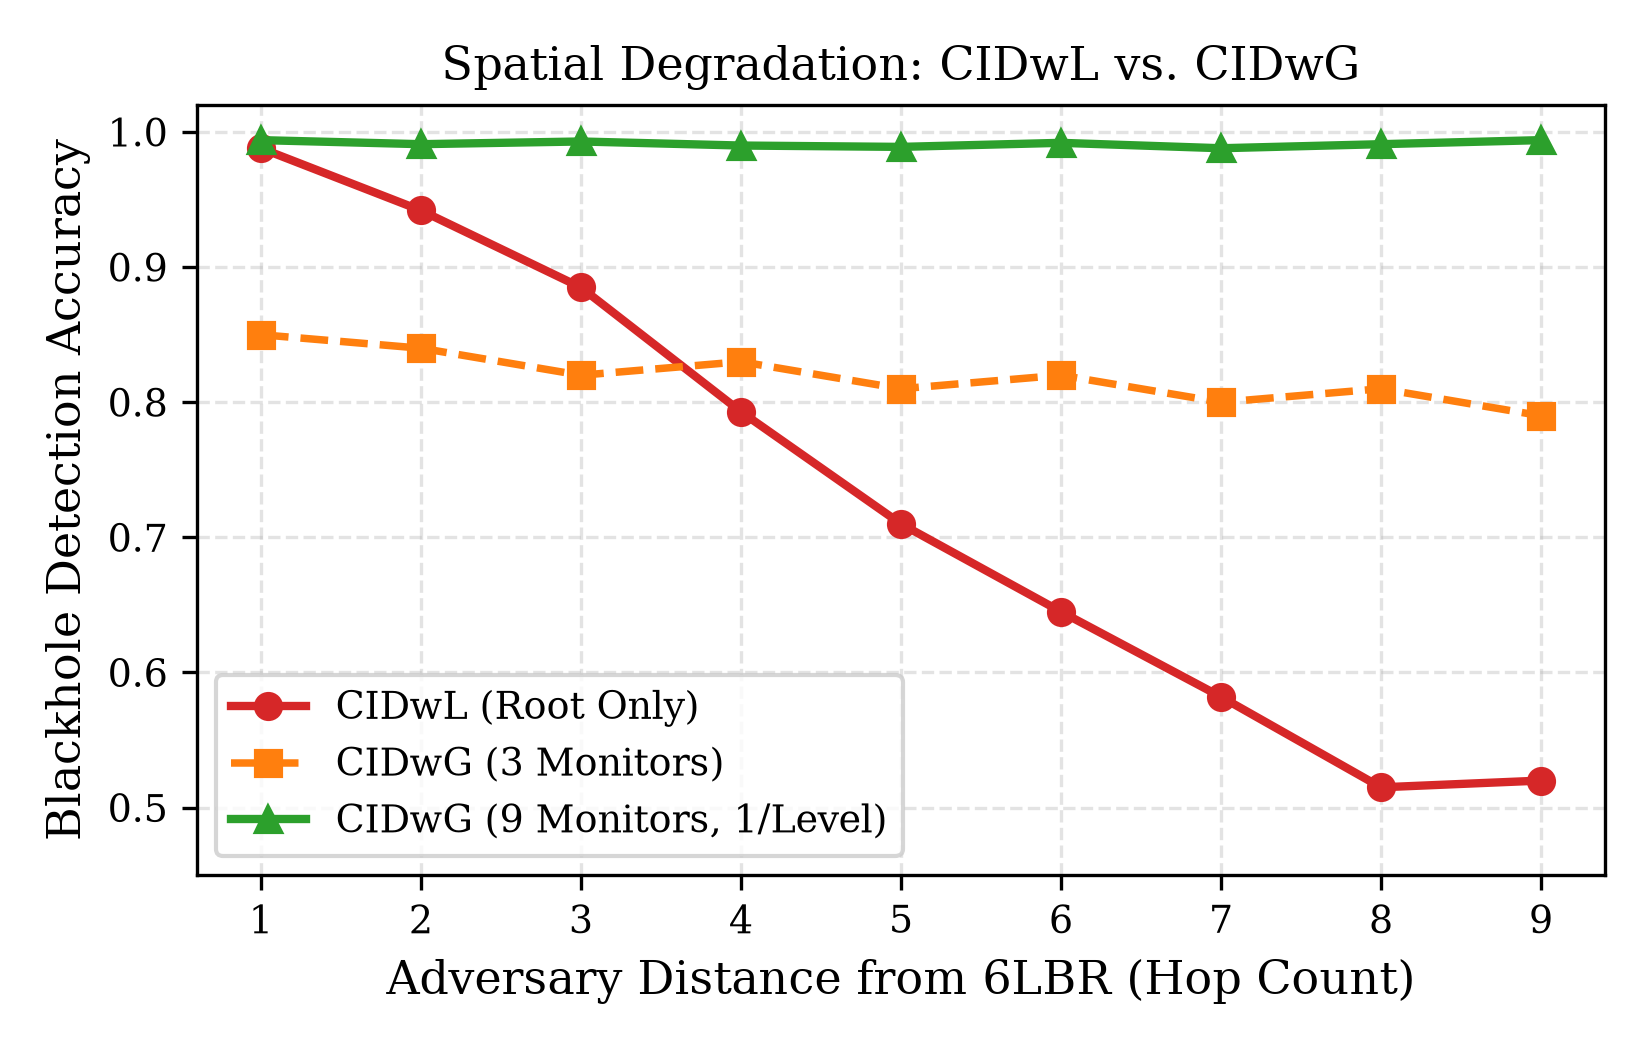
\includegraphics[width=\textwidth]{images/fig4_cidwl_vs_cidwg_accuracy.png}
        \caption{Overall accuracy: CIDwL vs. CIDwG with 2--9 nodes \cite{yilmaz2025exploring}.}
      \end{figure}
    \end{column}
  \end{columns}
\end{frame}

% ==============================================================================
% SLIDE 10: DISCUSSION
% ==============================================================================
\section{Discussion}
\begin{frame}{Discussion: Multi-Criteria Architectural Trade-offs}
  \begin{table}[h]
    \centering
    \scriptsize
    \caption{Comprehensive Qualitative \& Quantitative Architectural Comparison \cite{yilmaz2025exploring}}
    \begin{tabular}{lcccc}
      \toprule
      \textbf{Evaluation Metric} & \textbf{CIDwL} & \textbf{CIDwG} & \textbf{DCID} & \textbf{FedID (Proposed)} \\
      \midrule
      \textbf{Detection Accuracy} & Poor (51\%--71\%) & High (71\%--99\%) & Moderate-High & \textbf{High (82\%--100\%)} \\
      \textbf{Runtime Comm. Overhead} & \textbf{0 Bytes} & $378 \times 10^3$ Bytes & 2,700 Bytes & \textbf{0 Bytes (Autonomous)} \\
      \textbf{Training Comm. Cost} & 0 Bytes & $378 \times 10^3$ Bytes & 2,700 Bytes & $37.8 \times 10^3$ Bytes (10\%) \\
      \textbf{Mote Energy Depletion} & \textbf{None} & Extreme (Channel load) & Moderate (Local inf.) & \textbf{Negligible in Testing} \\
      \textbf{Single Point of Failure} & High Vulnerability & High Vulnerability & Resilient (Voting) & \textbf{Resilient (Edge Deployable)} \\
      \textbf{Data Privacy} & High (Local only) & Low (Raw feature leak) & Moderate (Alarms) & \textbf{High (Weights only)} \\
      \textbf{Packet Loss Tolerance} & High & Low (Loss degrades model) & Moderate & \textbf{High (Inference local)} \\
      \bottomrule
    \end{tabular}
  \end{table}
  \begin{alertblock}{Key Insight}
    CIDwG achieves high accuracy at the cost of network collapse. DCID reduces communication via voting (50\% majority is optimal) but increases local CPU workload. \textbf{FedID bridges this gap}.
  \end{alertblock}
\end{frame}

% ==============================================================================
% SLIDE 11: RESULTS PART 2
% ==============================================================================
\section{Results: FedID \& Novelty}
\begin{frame}{Results (Part 2): Proposed FedID \& Novelty Extension}
  \begin{columns}[T]
    \begin{column}{0.48\textwidth}
      \textbf{FedID Performance Highlights:}
      \begin{itemize}\scriptsize
        \item \textbf{Flower + XGBoost} implementation with FedAvg.
        \item \textbf{Data Sharing Ratio ($S$):} Sharing 10\% of samples eliminates non-IID divergence (cosine similarity $>0.9$).
        \item FedID outperforms CIDwL across all attacks: BH (95.7\%), SF (82.4\%), DI (87.0\%), DR (82.6\%), HF (98.0\%), IV (100\%), WP (87.4\%).
        \item \textbf{CICIoT2023 Benchmark:} 99.60\% Binary Accuracy, 98.80\% Multiclass Accuracy (outperforming MLP and LSTM).
      \end{itemize}
      \begin{figure}
        \centering
        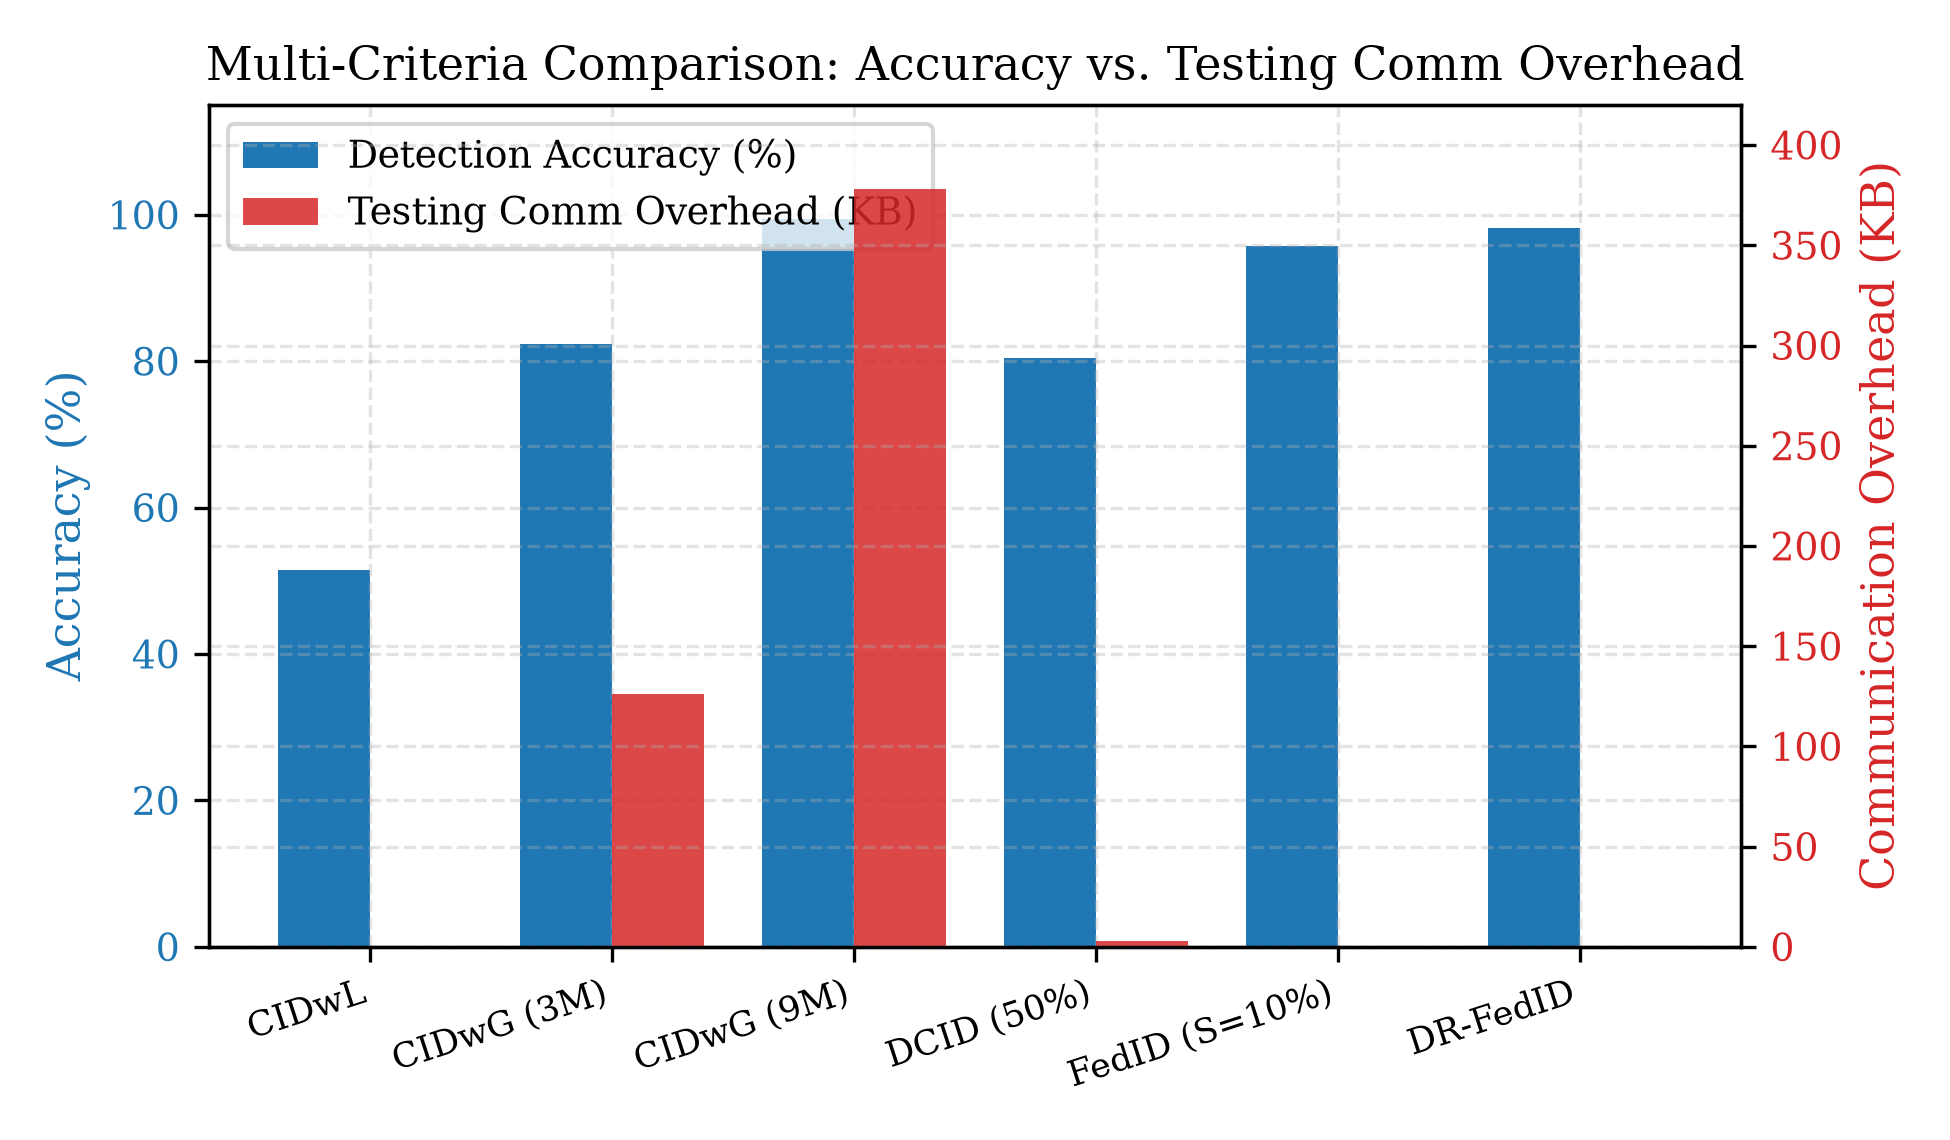
\includegraphics[width=0.95\textwidth]{images/fig7_fedid_vs_architectures_accuracy.png}
        \caption{FedID accuracy vs. baselines across attacks \cite{yilmaz2025exploring}.}
      \end{figure}
    \end{column}
    \begin{column}{0.5\textwidth}
      \textbf{Upcoming Iteration: Novel Extension (DR-FedID):}
      \begin{figure}
        \centering
        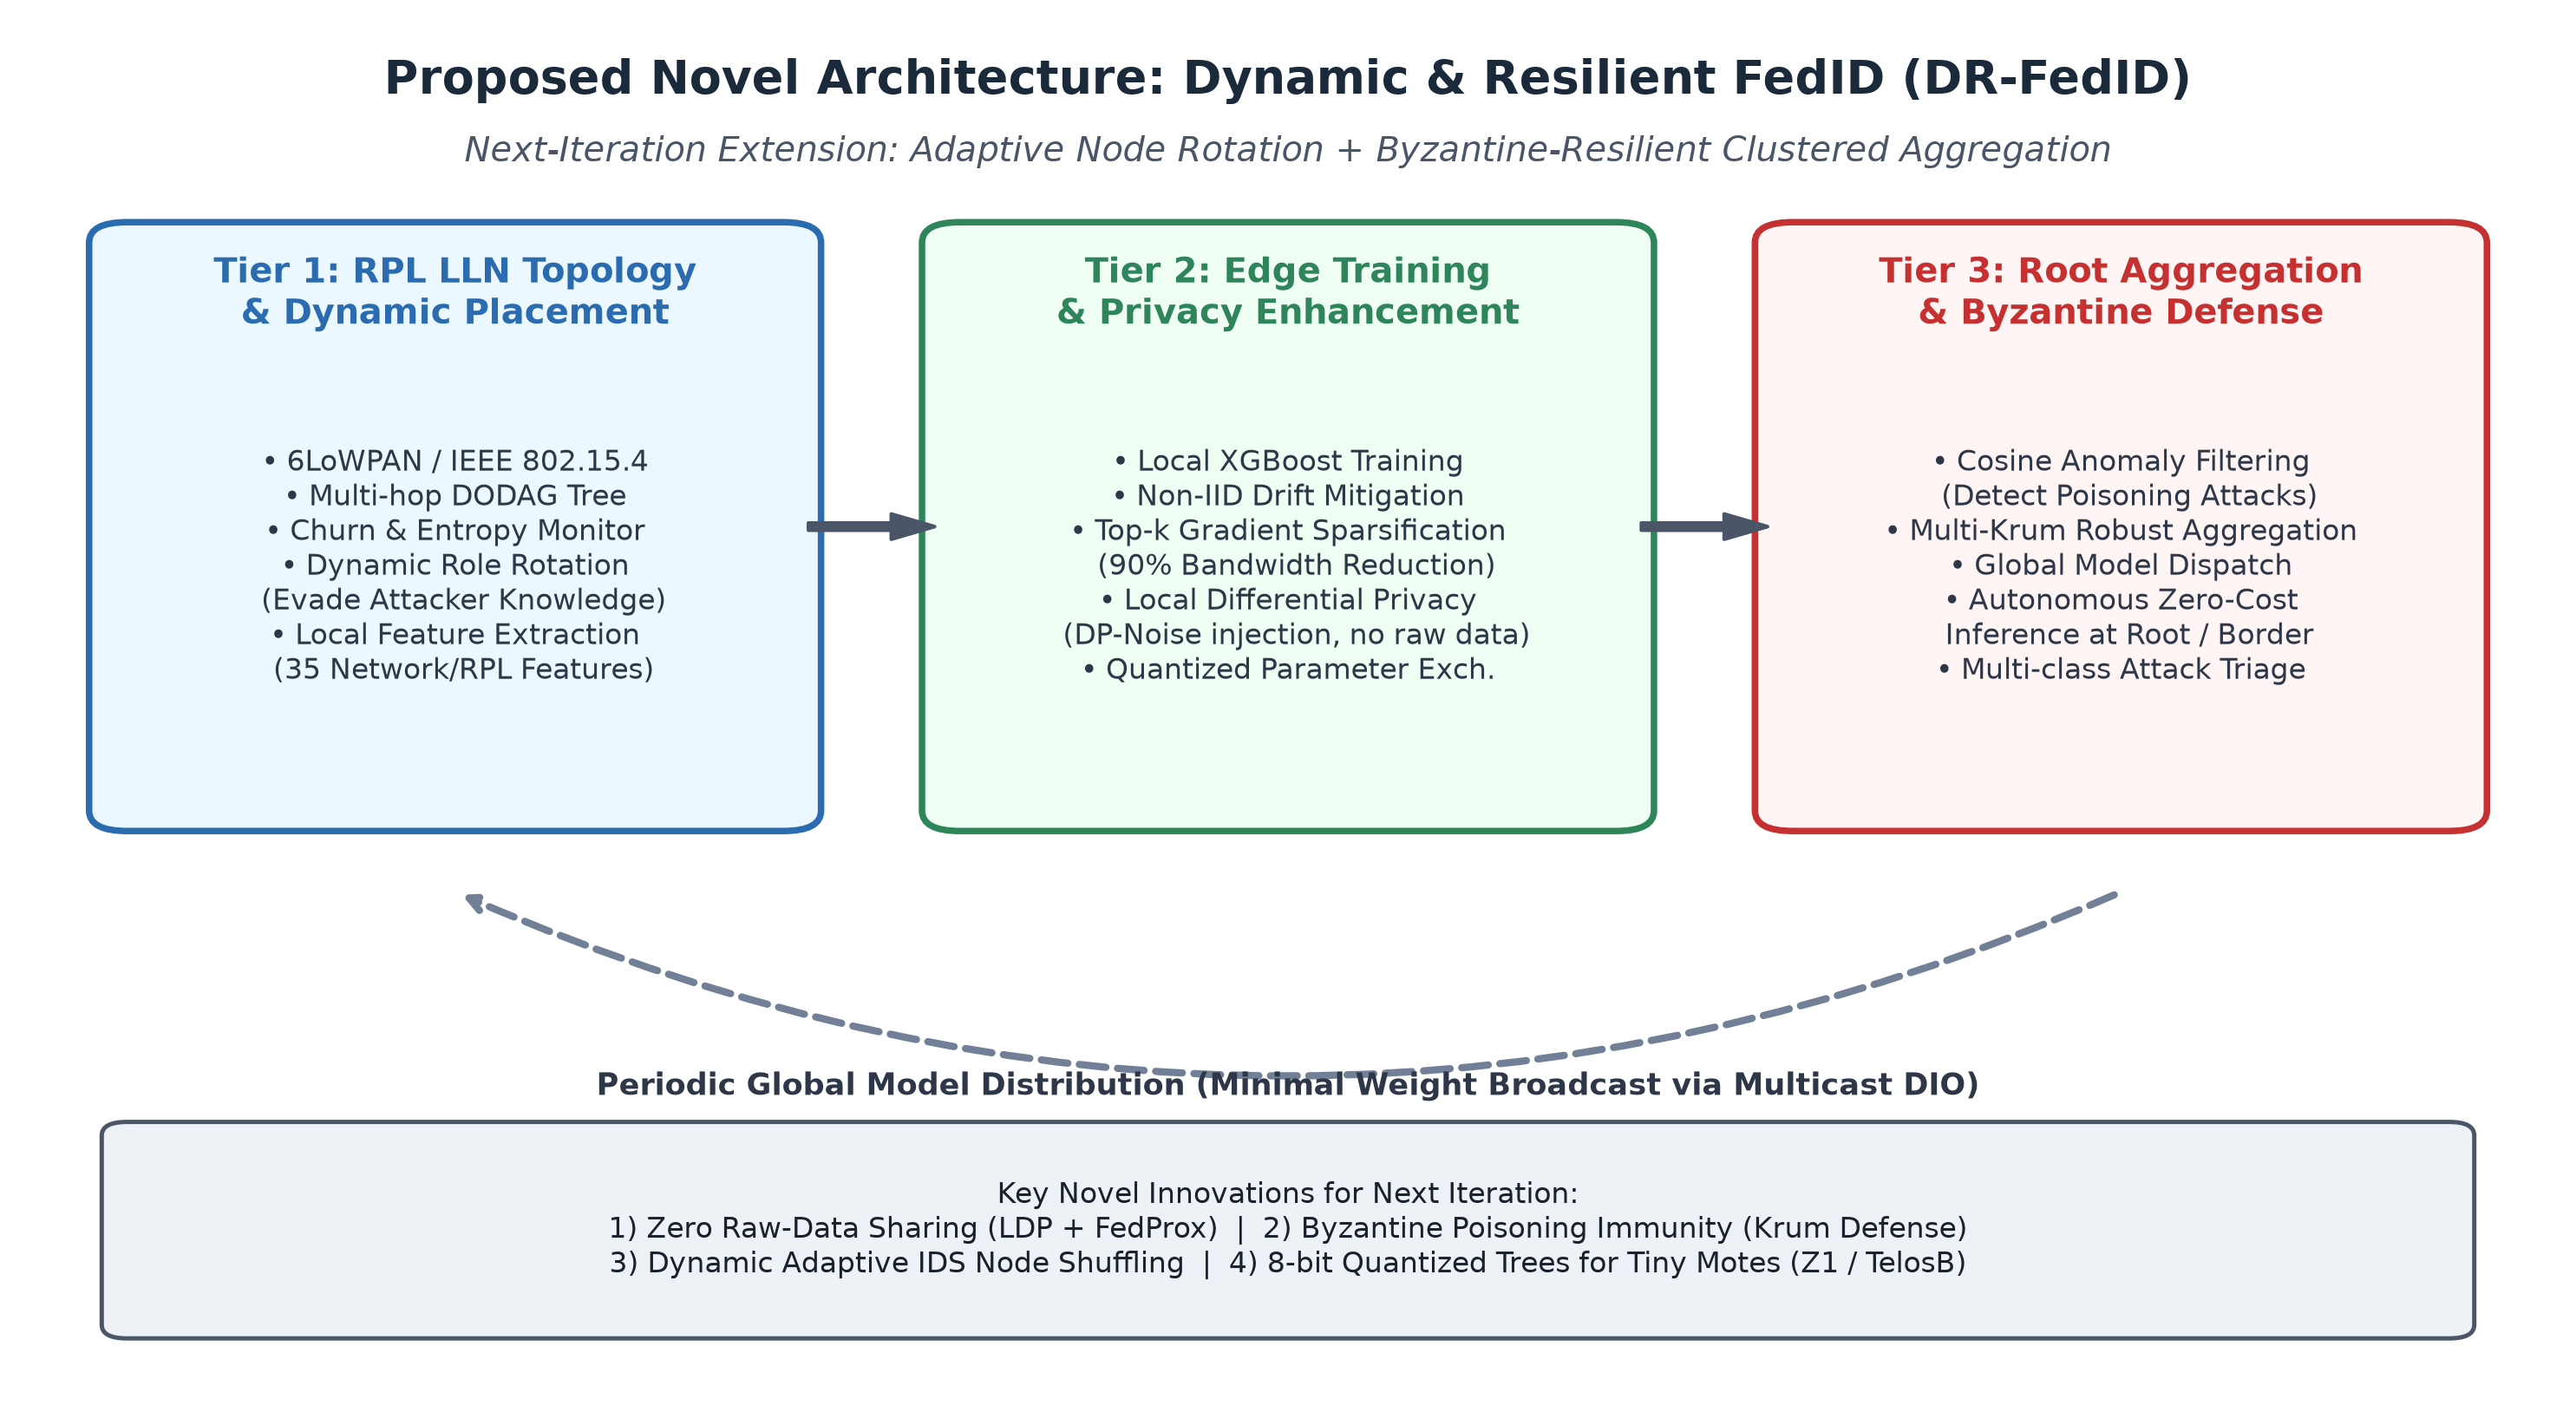
\includegraphics[width=\textwidth]{images/novelty_architecture.png}
        \caption{Proposed Novel Framework: Dynamic Placement \& Byzantine Defense.}
      \end{figure}
      \begin{itemize}\scriptsize
        \item \textbf{Dynamic Placement:} Entropy/routing-churn monitor dynamically rotates collaborator roles, neutralizing attacker evasion.
        \item \textbf{Zero-Leakage Privacy:} Local Differential Privacy ($\epsilon, \delta$-LDP) replaces raw sample sharing.
        \item \textbf{Byzantine Resilience:} Multi-Krum / Cosine-filtering rejects poisoned gradients from insider adversaries.
      \end{itemize}
    \end{column}
  \end{columns}
\end{frame}

% ==============================================================================
% SLIDE 12: CONCLUSION & FUTURE WORK
% ==============================================================================
\section{Conclusion \& Future Work}
\begin{frame}{Conclusion \& Future Roadmap}
  \begin{columns}[T]
    \begin{column}{0.5\textwidth}
      \begin{block}{Project Conclusions}
        \begin{itemize}\footnotesize
          \item \textbf{Placement is Decisive:} IDS efficacy in RPL is fundamentally dictated by physical/topological distance from the adversary.
          \item \textbf{Centralized Failure:} Single-node root monitoring (CIDwL) leaves deep network tiers completely unprotected.
          \item \textbf{FedID Superiority:} Federated Learning achieves multi-hop detection accuracy comparable to global streaming while maintaining \textbf{0-byte runtime communication overhead}.
          \item Resolves the non-IID dilemma in IoT with minimal sample coordination ($S=10\%$).
        \end{itemize}
      \end{block}
    \end{column}
    \begin{column}{0.48\textwidth}
      \begin{block}{Future Research Directions}
        \begin{itemize}\footnotesize
          \item \textbf{Adaptive Dynamic Scheduling:} Implement reinforcement learning (Q-learning) on nodes to adaptively schedule training rounds based on energy harvest rates.
          \item \textbf{Cross-Layer Feature Fusion:} Integrate MAC-layer retransmissions (IEEE 802.15.4 ACK failures) and PHY RSSI jitter for early wormhole localization.
          \item \textbf{Hardware Testbed Deployment:} Validate DR-FedID on physical testbeds (e.g., FIT IoT-LAB with Cortex-M3 nodes).
        \end{itemize}
      \end{block}
    \end{column}
  \end{columns}
\end{frame}

% ==============================================================================
% SLIDE 13: REFERENCES
% ==============================================================================
\section{References}
\begin{frame}[allowframebreaks]{References}
  \footnotesize
  \bibliographystyle{IEEEtran}
  \bibliography{references}
\end{frame}

% ==============================================================================
% SLIDE 14: THANK YOU SLIDE
% ==============================================================================
\section{Q\&A}
\begin{frame}{Thank You!}
  \begin{center}
    \vspace{0.8cm}
    {\Huge \textbf{\textcolor{navyblue}{Thank You!}}}
    
    \vspace{0.6cm}
    {\large Questions \& Discussion}
    
    \vspace{0.8cm}
    \begin{tcolorbox}[colback=blue!5!white, colframe=navyblue, width=0.85\textwidth, halign=center]
      \textbf{Project Title:} Exploring and Enhancing Placement of IDS in RPL \\
      \textbf{Team 19:} Mohammadilyas Patel, Shaik Sifat Ahmed, Abhinay \\
      \textbf{Institution:} IIITDM Kancheepuram (Chennai 600127) \\
      \textbf{GitHub Repository:} \url{https://github.com/mdilyas-27/cns_project_team19}
    \end{tcolorbox}
    
    \vspace{0.4cm}
    \footnotesize
    \textit{Overleaf Project Package \& Complete Codebase Available for Replication.}
  \end{center}
\end{frame}

\end{document}

